\begin{figure}[!htb]
    \center
        \begin{tikzpicture}
            \Vertex[x=0.5, y=0.5,color=white,opacity=0.5,label=p, size=1, shape=circle]{p}
            \Vertex[x=-1,y=3,color=white,opacity=0.5,label=q, size=1, shape=circle]{q}
            \Vertex[x=2,y=2.5,color=white,opacity=0.5,label=r, size=1, shape=circle]{r}
            \Vertex[x=4,y=4,color=white,opacity=0.5,label=s, size=1, shape=circle]{s}
            \Vertex[x=2.5,y=6.5,color=white,opacity=0.5,label=t, size=1, shape=circle]{t}
            \Vertex[x=5.5,y=1.75,color=white,opacity=0.5,label=u, size=1, shape=circle]{u}
            \Vertex[x=7.5,y=4,color=white,opacity=0.5,label=v, size=1, shape=circle]{v}
            \Vertex[x=7.5,y=6.5,color=white,opacity=0.5,label=w, size=1, shape=circle]{w}
            \Edge[label=\textcolor{black}{$20$}, color=tuorange](q)(r)
            \Edge[label=\textcolor{black}{$17$}, color=tuorange](p)(r)
            \Edge[label=\textcolor{black}{$15$}, color=tuorange](r)(s)
            \Edge[label=\textcolor{black}{$9$}, color=tuorange](w)(s)
            \Edge[label=\textcolor{black}{$3$}, color=tuorange](u)(s)
            \Edge[label=\textcolor{black}{$8$}, color=tuorange](t)(s)
            \Edge[label=\textcolor{black}{$4$}, color=tuorange](v)(s)
            \Edge[label=\textcolor{black}{$2$}, color=tugray](r)(t)
            \Edge[label=\textcolor{black}{$1$}, color=tugray](r)(u)
            \Edge[label=\textcolor{black}{$6$}, color=tugray](q)(t)
            \Edge[label=\textcolor{black}{$3$}, color=tugray](v)(w)
            \Edge[label=\textcolor{black}{$5$}, color=tugray](w)(t)
            \Edge[label=\textcolor{black}{$1$}, color=tugray](u)(v)
            \Edge[label=\textcolor{black}{$5$}, color=tugray](q)(p)
            \Edge[label=\textcolor{black}{$2$}, color=tugray](p)(u)
            \end{tikzpicture}
    \caption[Chow-Liu algorithm maximum spanning tree visualization.]{Weighted graph G=(V,E), where each weight is the mutual information between two random variables. The edges used for the maximum spanning tree are colored orange, which has a total weight of 76. While the original graph is usually fully connected, some edges have been omitted for better visibility. We assume that the missing edges each have a weight of 0.}
    \label{fig:mst}
\end{figure}